\documentclass[a4paper]{article}

\usepackage{hyperref}
%\hypersetup{
%colorlinks=false,              % bool: Liens colorés
%pdfborder={0 0 0}             % Ne pas encadrer les liens
%}
\usepackage[utf8]{inputenc}  
\usepackage[francais]{babel}  
\usepackage[top=2cm, bottom=2cm, left=2cm, right=2cm]{geometry}
\usepackage{graphicx}
\usepackage[final]{pdfpages} 
\usepackage{rotating}
\usepackage{float}

\newcommand{\jeua}{countries2007\_ALL }
\newcommand{\jeub}{countries2007\_NoMissing1 }
\newcommand{\jeuc}{countries2007\_NoMissing2 }
\newcommand{\lesite}{\textit{The world bank}}
% définir les commandes ici

% s'il y a beaucoup de commandes et de packages à inclure n'h&ésitez pas
% à mettre tout ça dans un fichier include.tex et l'inclure
% \input{include.tex}


\begin{document}
\begin{titlepage}
\begin{center}
 
 \vfill
		\begin{Large}\textbf{Hexanome 4211 :} 
		Elisa \bsc{Abidh}, Gaël \bsc{Motte}\end{Large}
		
\vfill
	
		\begin{Huge}
		Data Mining : Rapport \\
		\end{Huge} 

\vfill
	
		 
		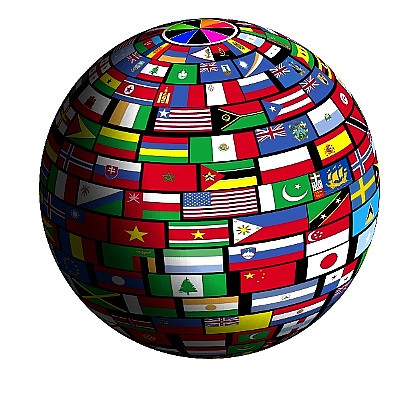
\includegraphics[scale=0.3]{Image/drapeaux-du-monde}
\begin{Large}
		
		
		Jeu de données :  \textit{Countries2007}\\
		\end{Large}

\vfill		
		\begin{Large}
		Mars 2011
		\end{Large}
		
\includegraphics[scale=0.1]{Image/creative_commons}
	\end{center}
	

\end{titlepage}
%----------------------------------------------------

%--------------------------------- Table des matières
\newpage
\tableofcontents
\newpage
%----------------------------------------------- Plan

\input{intro.tex}

\part{Découverte du jeux de données et pré-traitement}
\section{Découverte}
Le jeu de données traite un bon nombre des indicateurs les plus utilisés lors des analyses géographiques pour de nombreux pays.\\
Ces données proviennent du site \lesite.\\
Sur ce site, nous obtenons d'ailleurs une bonne description de ce que signifient les différents indicateurs. %DONE

%remarques sur le jeu en lui même, la décomposition en
\section{Traitements préliminaires}

\subsection{Union Européenne}
L'union européenne étant un ensemble de pays qui nous sont assez bien connus, dans leurs grandes caractéristiques économique et sociétales, nous avons estimé qu'il était intéressant de les indiquer de façon claire.\\
Nous avons donc effectué un premier traitement consistant à ajouter un attribut à tous les enregistrements, indiquant si ils appartiennent à l'union européenne ou non.\\

\subsubsection{Valeurs Brutes}
Deux problèmes se posent dans le cas des valeurs brutes : 
\paragraph{Disproportions} Dans le cas de valeurs brutes telles que la surface ou le PIB, des disproportions sont flagrantes et déformes à elle seule l'analyse. Ces critères, quand ils sont utilisés de manière brute deformes les résultats.\\
Pour résoudre ce problème, nous proposons d'établir de nouveaux attributs qui permettent d'obtenir des valeurs relatives : 
\begin{itemize}
	\item Population density 
	\item GDP per inhabitant
\end{itemize}

\paragraph{Normalisation}
Afin de permettre la comparaison des différents enregistrements, et surtout des différents attributs, il est indispensable que ceux-ci soient normalisés.
Dans la suite, nous utiliserons la normalisation par Z-score.







 %DONE
%ajout de la classe UE, NON UE.

\section{Adaptations du jeu de données}

Une étape indispensable à la fouille de donnée réside dans le choix des attributs qui seront utilisés pour l'étude.
Il nous font donc y prêter une attention particulière, et choisir ceux qui nous paraissent les plus utiles, et essayer de réduire les dimensions et axes d'études.

\subsection{Corrélation d'attributs}

Afin de réduire les dimensions de l'étude, nous cherchons les corrélations entre les attributs disponibles. Voici les résultats pour le jeu \jeuc.

\begin{figure}[H]
	\begin{center}
		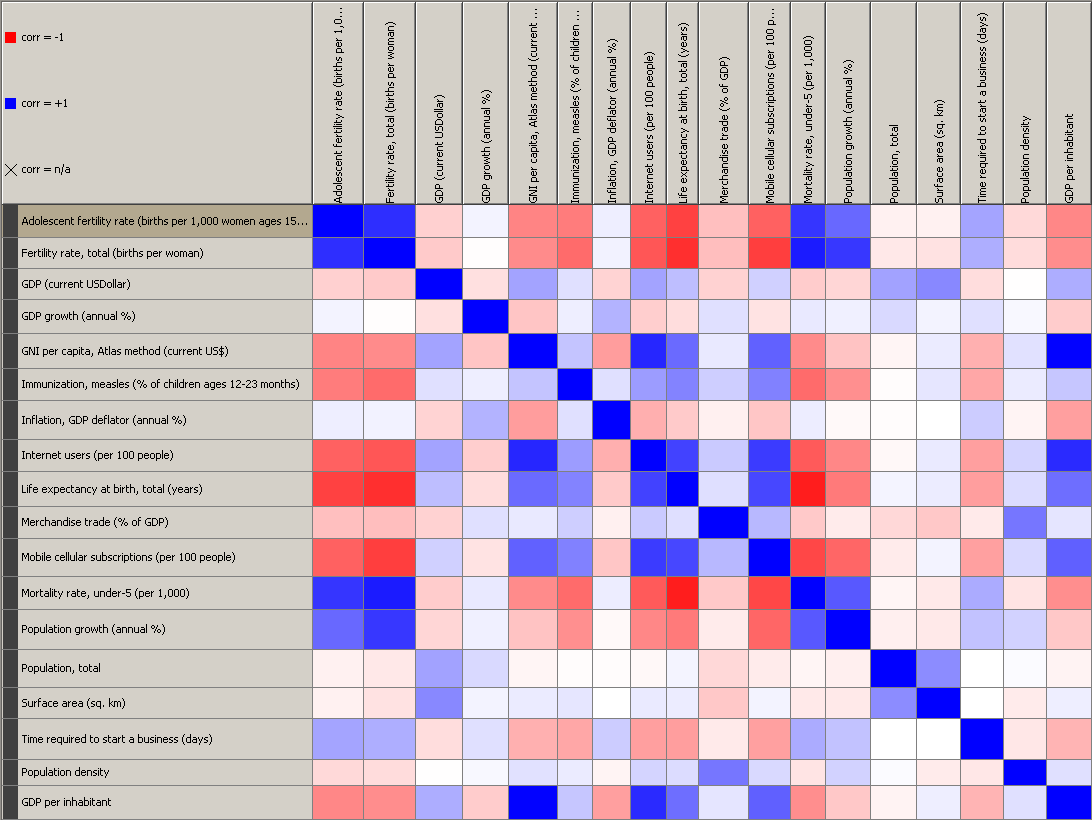
\includegraphics[scale=0.5]{Image/MatriceCorrelationNoMissing2}
		\caption{Matrice de corrélation pour le jeu \jeuc}
	\end{center}
\end{figure}

\subsection{Réduction des dimensions}

Au vu de ces résultat, nous estimons qu'une corrélation de 75\% minimum doublée d'une sémantique forte peut justifier la réduction de dimension. Nous utiliserons pour cela le compostant PCA.
 
Nous avons donc effectué les rapprochements suivants : 
\paragraph{Infrastructure} corrélation : 77\%
		\begin{itemize}
			\item Mobile cellular subscriptions
			\item Internet users
		\end{itemize}
\paragraph{population youth} corrélation : 83\%
		\begin{itemize}
			\item Adolescent fertility rate
			\item Fertility rate
			\item Mortality rate under 5 years
		\end{itemize}
\hfill\\

De plus nous observons que certains attributs sont quelque peu redondants. Par exemple, GDP per Inhabitant (créé par nos soins) et GDI per capita sont corrélés à plus de 99\%. Nous n'utiliserons donc que ce second attribut, donné par \lesite .



 %DONE
%expliquer comment on a reduit la dimmension,
   % methode
   % corélation
   % nouveau nom
   
\section{Discrimination des outliers}
Les outliers sont des valeurs qui se situent dans des valeurs extrêmes qui empêchent d'obtenir un modèle cohérent.\\
Il est donc important de les identifier et de les exclure pour la suite de l'étude.

\subsection{Méthode de recherche des outliers}

\paragraph{Box Plot}
Pour rechercher les outliers présents dans le jeu de données, une méthode peut consister à regarder des diagrammes en boites à moustaches.
Les valeurs extrêmes apparaissent clairement.

\begin{figure}[H]
	\begin{center}
		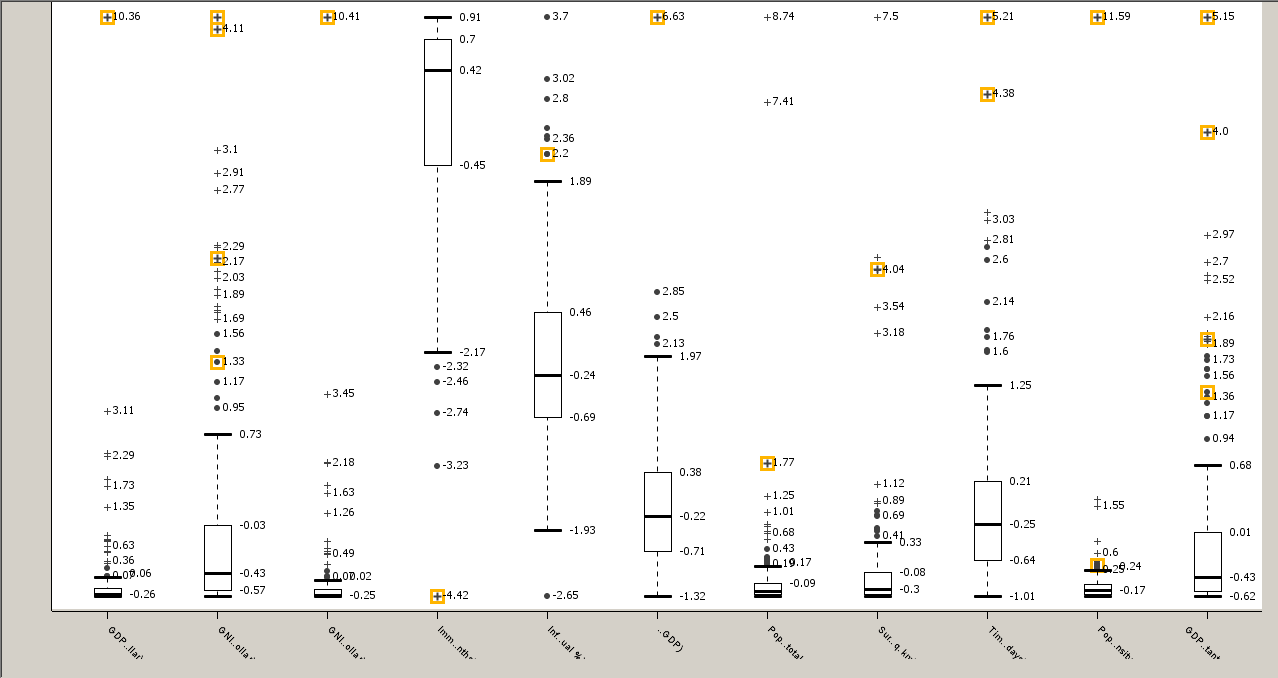
\includegraphics[scale=0.5]{Image/BoxplotOutlierNoMissing2}
		\caption{Diagrammes de boite à moustaches pour le jeu \jeuc}
	\end{center}
\end{figure}

\paragraph{Hierachical trees}
Un autre axe de recherche de ces outliers peut être d'utiliser des clusterisation hiérarchique en mode SINGLE qui font apparaitre les entrées dont les distances sont grandes de façon claires.


\begin{figure}[H]
	\begin{center}
		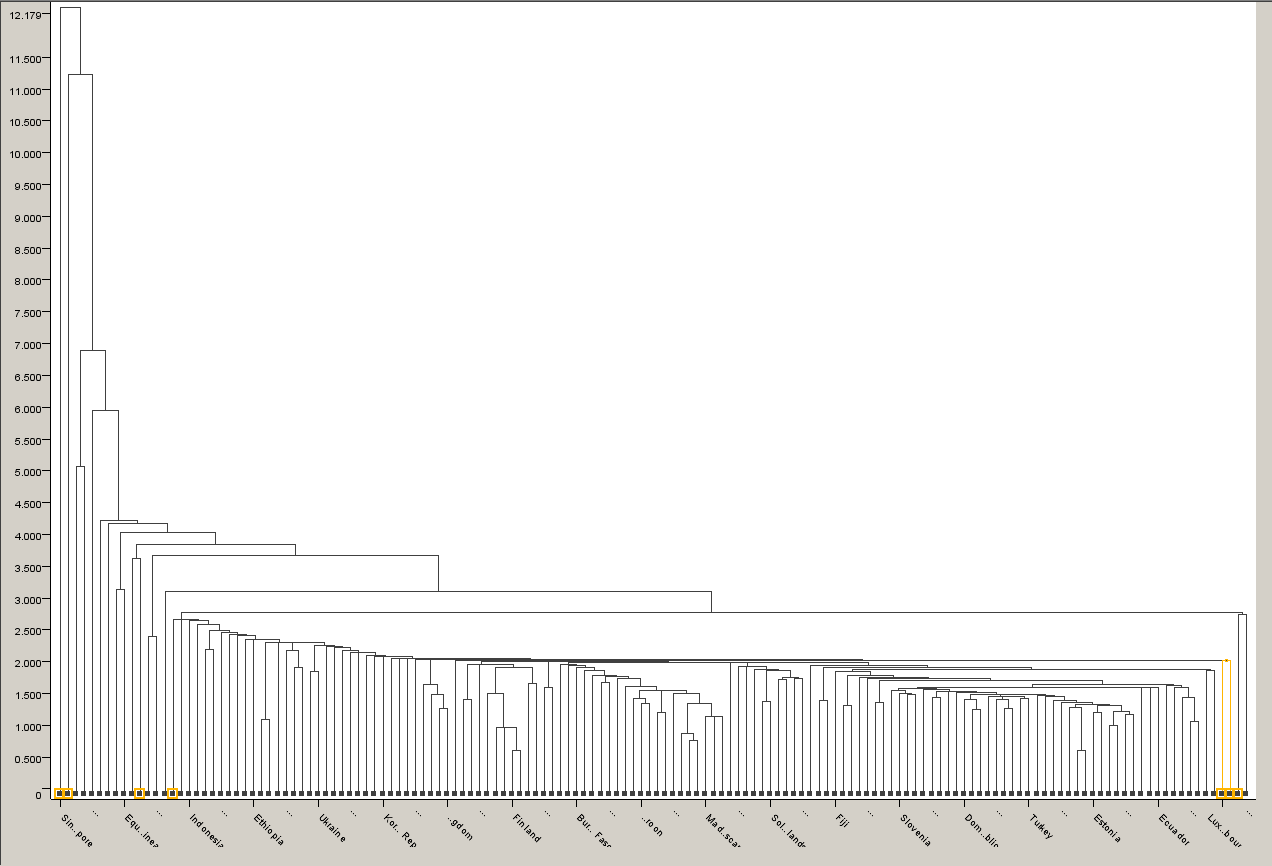
\includegraphics[scale=0.5]{Image/DendogrammeOutliers}
		\caption{Diagrammes de boite à moustaches pour le jeu \jeuc}
	\end{center}
\end{figure}
%hierachical tree en mode single pour trouver les distances "anormales"

\subsection{Outliers écartés}

\paragraph{Hierachical tree} Ces deux pays doivent être écartés au vu des résultats du clustering hiérarchique. On comprend également que ce sont dans le monde deux exceptions : 
\begin{itemize}
	\item \textbf{USA} : Une taille exceptionnelle, et la richesse de 50 états
	\item \textbf{Singapour} : Cité état à la densité de population et a la richesse par habitant hors norme 
\end{itemize}

\paragraph{BoxPlot}
Le diagramme en boite à moustache montre plusieurs exceptions : 
\begin{itemize}
	\item \textbf{Chad} : Immunisation contre la rubéole exceptionnellement faible
	\item \textbf{Guinée-bisseau} : Il semble difficile de démarrer une entreprise en Guinée-Bissau
	\item \textbf{Luxembourg} : PNB par habitant hors norme
	\item \textbf{Norvège} : PNB par habitant hors norme
\end{itemize}

%liste des outliers écartés
%DONE
%liste des outliers et raison pour lesquels on les a éliminés


  \newpage 
\part{Analyse du jeu de données}
\section{Axes de Recherche}
Après réflexion nous avons décidé de regrouper les attributs par catégorie d'indicateur. En effet nous préférons faire du clustering sur un groupe d'attribut plutôt que sur la totalité des attributs.
Pour faire ces groupes d'attributs nous avons pris comme référence le site de World Bank qui a lui même récolté les données. Nous avons dégagé deux indicateurs principaux : Santé et Politique économique. Pour le jeu de donnée 'no missing2', l'indicateur Santé regroupe les attributs suivant : Adolescent fertility rate, Fertility rate total, Immunization measles, Life expectancy at birth, Mortality rate under-5, Population growth et Population total; l'indicateur Politique économique regroupe lui les attributs: GDP, GDP growth, GNI per capita, atlas method et GNI, atlas method.\\
Les autres attributs ne seront pas traité dans la suite de l'analyse, nous avons fais le choix pour la suite de nous centrer uniquement sur les attributs cités plus haut.\\
Nous allons par la suite faire du clustering avec seulement les attributs de l'indicateur Santé puis uniquement les attributs Politique économique.
Le but cette réduction d'attributs est de voir si l'indicateur Santé et Politique économique permet de dégager des groupes de pays, de voir ou se situe l'Europe. Par la suite nous souhaitons étendre la recherche sur le grand jeu de donné. Pour le grand jeu de donnée nous supprimerons tous les pays dont les attributs qui nous intéresse ne sont pas renseignés. Nous justifions ce choix par le fait que nous ne savons pas ce que fais exactement Knime avec les données non renseignées. 


\section{Clustering hierachique}
TODO
%montrer les résultats  
   % dendrogramme
   % distance
   % conclusion sur le nb de clusters
\section{Clustering par partionement}
Nous avons réalisé le clustering par partitionnement à l'aide du composant hierarchical Clustering avec la configuration Linkage type : COMPLETE. Pour observer les résultats nous avons utilisé le composant Scatter Matrix.

\subsection{Santé}
Nous avions choisi de faire 3 clusters (cf section précédente), dont la répartitions des pays se fait comme suit : 

\begin{figure}[H]
	\begin{center}
		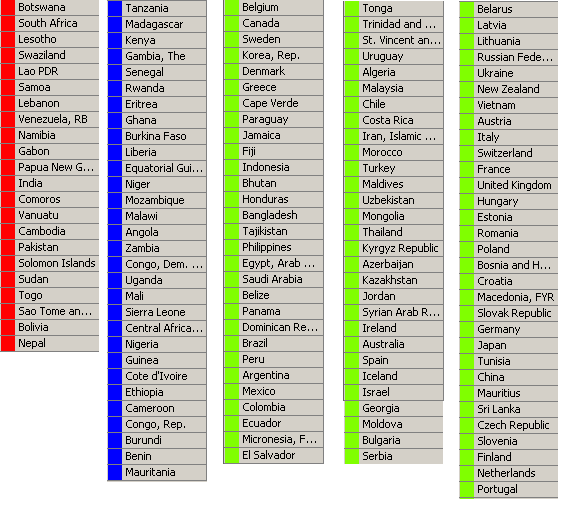
\includegraphics[scale=0.5]{Image/TableViewSanteNoMissing2}
		\caption{Liste des pays par clusters sur les critères de santé avec le jeu \jeuc}
	\end{center}
\end{figure}


Nous obtenons les résultats suivants : 

\begin{figure}[H]
	\begin{center}
		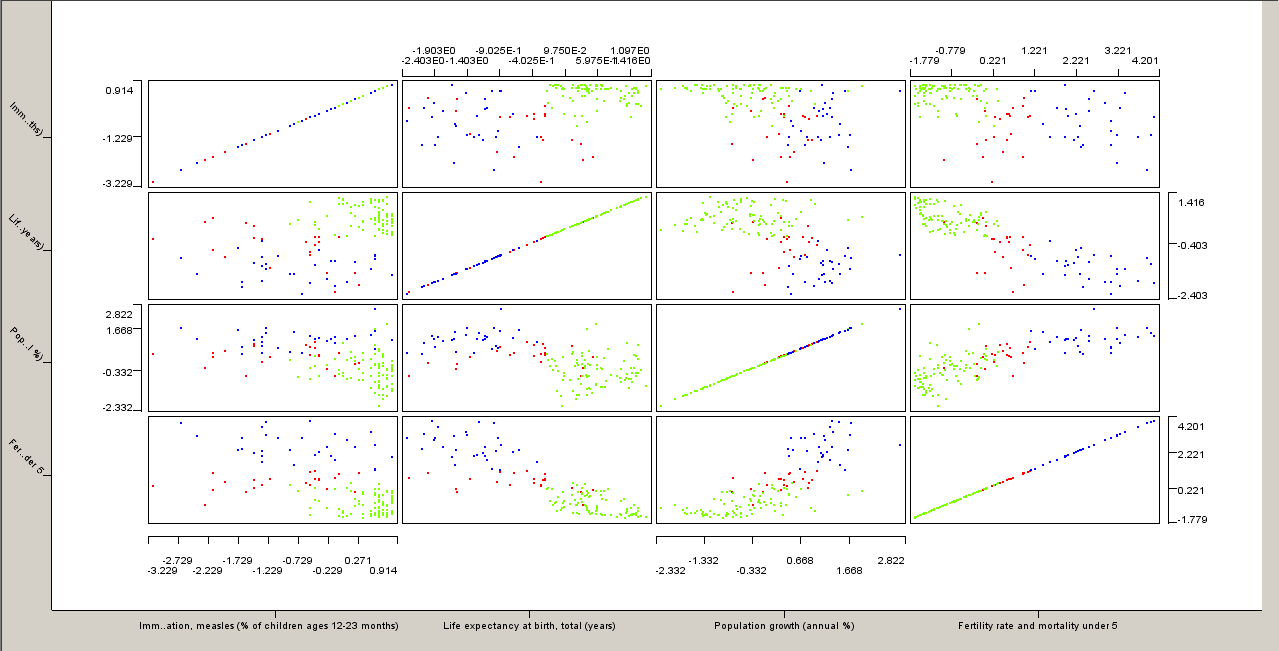
\includegraphics[scale=0.5]{Image/ScatterMatrixSanteNoMissing2}
		\caption{Scatter Matrix des attributs de l'indicateur Santé \jeuc}
	\end{center}
\end{figure}

\paragraph{Analyse}
TODO : si j'ai bien compris c'est plutot cool :)

\subsection{Économie}
Au vu des distances obtenues dans la section précédente, nous obtenons 4 clusters.

\begin{figure}[H]
	\begin{center}
		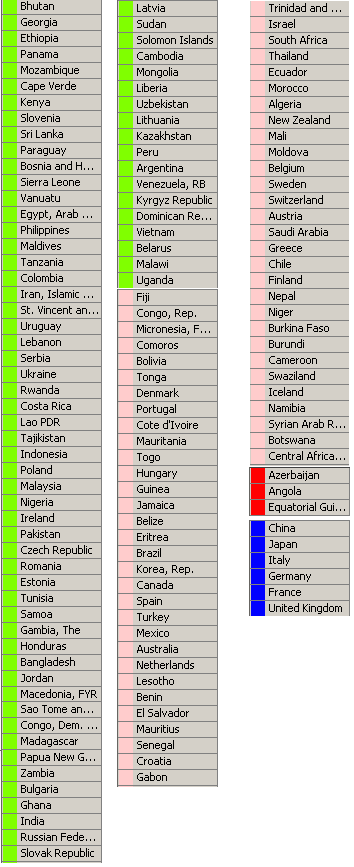
\includegraphics[scale=0.5]{Image/TableViewPolitiqueNoMissing2}
		\caption{Liste des pays par clusters sur les critères économiques avec le jeu \jeuc}
	\end{center}
\end{figure}


Nous obtenons les résultats suivants : 

\begin{figure}[H]
	\begin{center}
		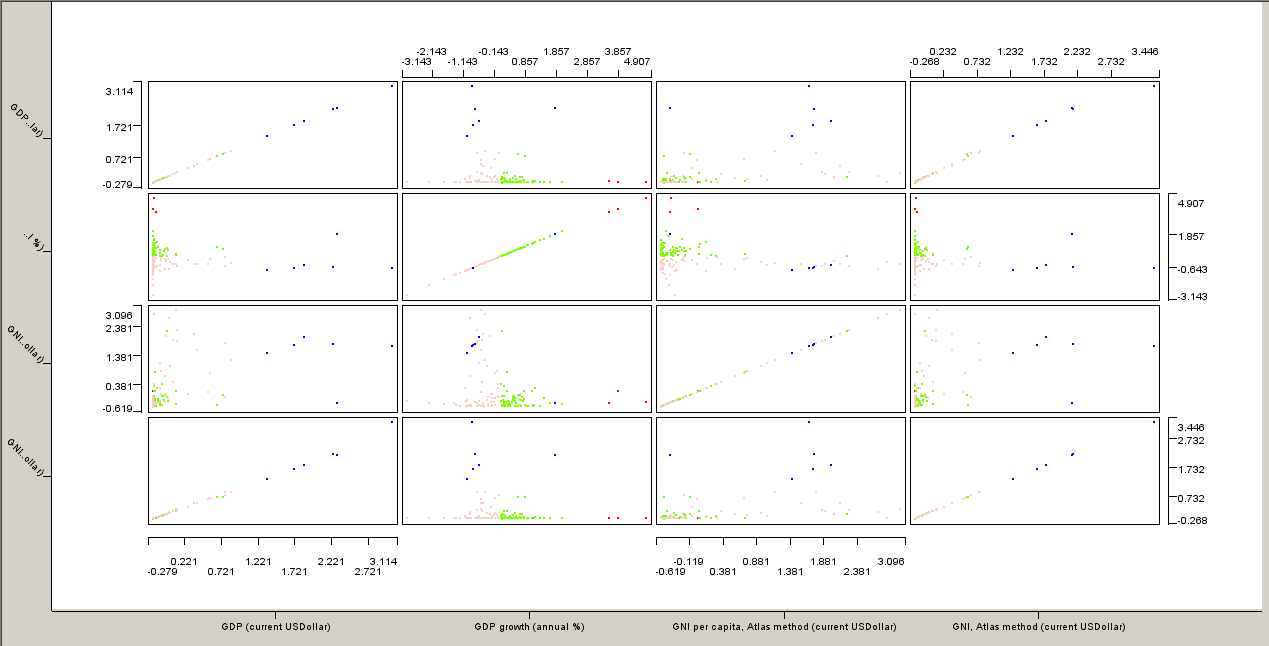
\includegraphics[scale=0.5]{Image/ScatterMatrixPolitiqueNoMissing2}
		\caption{Scatter Matrix des attributs de l'indicateur de politique économique \jeuc}
	\end{center}
\end{figure}

\paragraph{Analyse}
TODO : si j'ai bien compris c'est pas clair :)




% liste des attributs qui servent a partitioner
   % pourquoi
   % resultats

\newpage
\part{Projet - UE et ses nouveaux membres en 2007}
\section{Introduction}
TODO
% idéee de justification de l'idée
\section{Méthodlogie suivie}
TODO
% reprise de ce qui été produit

\section{Validation des modèles}


\subsection{Classification supervisée}
Afin de mettre place des modèles utilisables et de qualité certaine, nous utiliserons la classification supervisée.\\
Nous nous attaquerons donc en priorité à l'union européenne et tacherons de vérifier si les résultats sont probants.

\paragraph{Santé}

\paragraph{Economie}

\subsection{Cross validation et stabilité}

\paragraph{Hierachical tree}

\paragraph{K-means}

\paragraph{K-nearest neighbor}
   % cross validation
   
\section{Résultats obtenus}
En appliquant le même arbre de décision, nous obtenons les résultats suivants
\begin{figure}[H]
	\begin{center}
		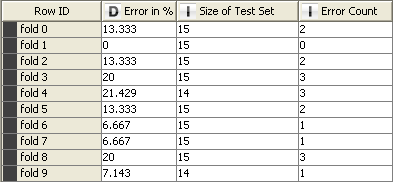
\includegraphics[scale=0.5]{Image/ErrorRatesSante}
		\caption{Resultats de la prédiction appliquée à la Roumanie et à la Bulgarie}
	\end{center}
\end{figure}
% présentation des resultats
\section{Conclusion sur le projet}
Nous avons trouvé ce projet intéressant car il nous permettait d'être créatif tout en gardant une méthodologie rigoureuse. Créatif car nous avions à notre disposition un jeu de données et c'était à nous de trouver des idées pour l'exploiter. Rigoureux car la fouille de donnée demande une méthodologie ainsi qu'un avis critique sur nos résultats.\\
Les principales difficultés rencontrées sont d'une part nous avons eu beaucoup de mal à partir une fois le jeu de données nettoyé. D'autre part l'analyse de nos résultats n'est pas évidente. Une fois face à nos résultats nous avions du mal à savoir si on pouvait réellement en tirer quelques choses.\\


% analyse critique de ce qu'on a fait 

\newpage
\part{Annexes : Workflows}
\begin{figure}[H]
	\begin{center}
		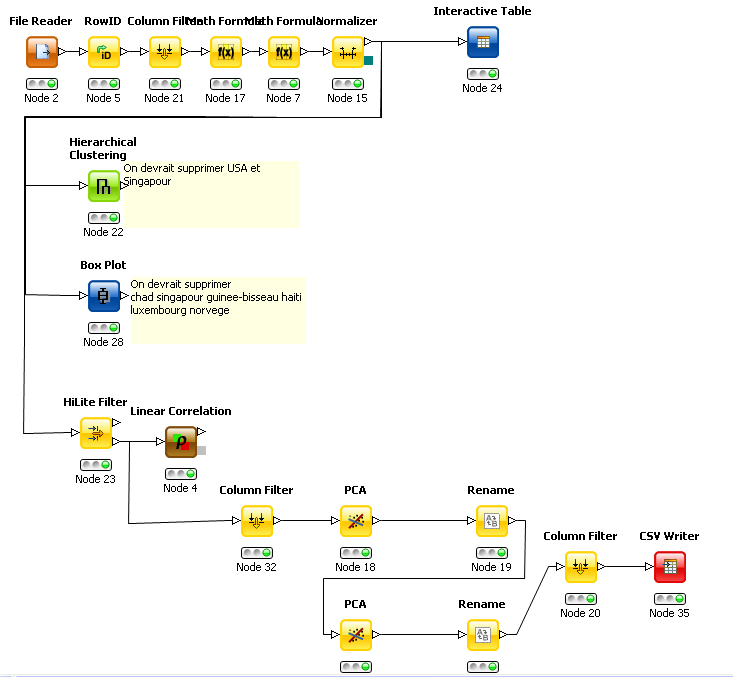
\includegraphics[scale=0.5]{Image/workflowOutlier}
		\caption{Workflow de recherche d'Outliers}
	\end{center}
\end{figure}
\begin{figure}[H]
	\begin{center}
		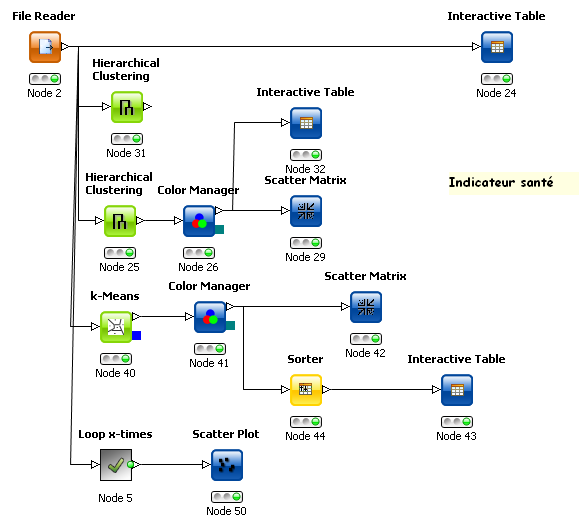
\includegraphics[scale=0.5]{Image/WorkflowClusteringSante}
		\caption{Workflow de recherche de cluster pour l'indicateur santé}
	\end{center}
\end{figure}
\begin{figure}[H]
	\begin{center}
		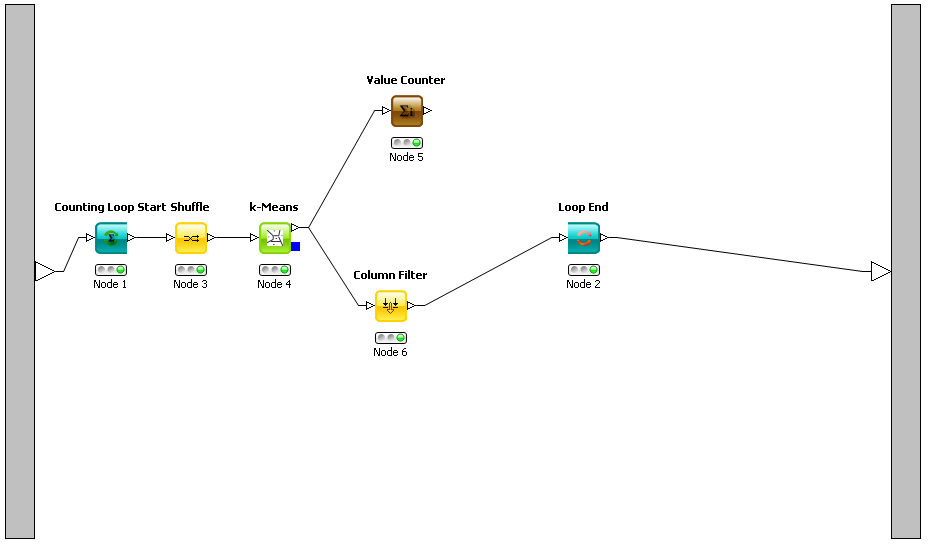
\includegraphics[scale=0.5]{Image/WorklowLoop}
		\caption{Workflow interne du Looper invalidant la stabilité de k-means}
	\end{center}
\end{figure}
\begin{figure}[H]
	\begin{center}
		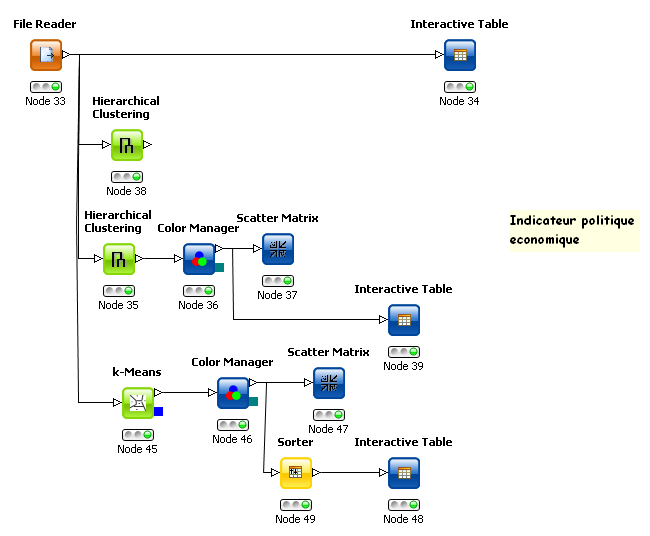
\includegraphics[scale=0.5]{Image/WorkflowClusteringSantePolitique}
		\caption{Workflow de recherche de cluster pour l'indicateur Politique Economique}
	\end{center}
\end{figure}
\begin{figure}[H]
	\begin{center}
		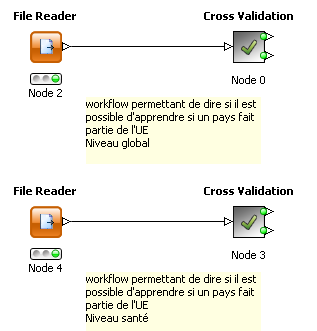
\includegraphics[scale=0.5]{Image/workflowValidation}
		\caption{Workflow de validation des modèles de Décision trees}
	\end{center}
\end{figure}
\begin{figure}[H]
	\begin{center}
		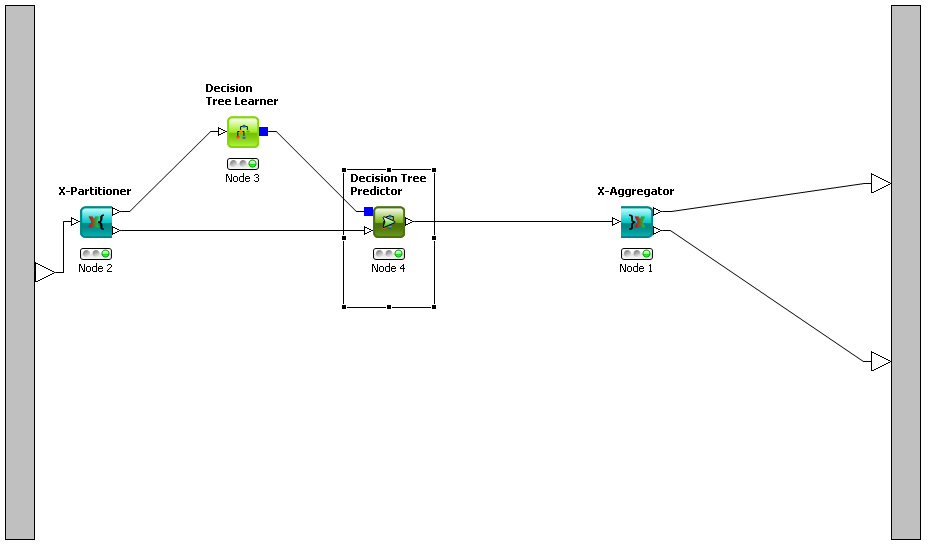
\includegraphics[scale=0.5]{Image/WorklowCrossValidationGlobal}
		\caption{Workflow interne du CrossValidation tous attributs confondus}
	\end{center}
\end{figure}
\begin{figure}[H]
	\begin{center}
		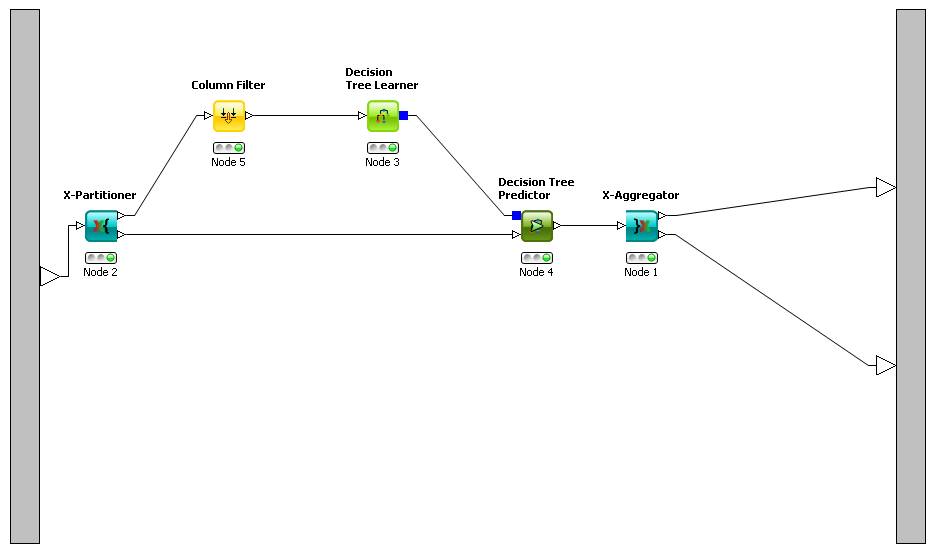
\includegraphics[scale=0.5]{Image/workflowValidatationSante}
		\caption{Workflow interne du CrossValidation pour l'indicateur santé}
	\end{center}
\end{figure}
\begin{figure}[H]
	\begin{center}
		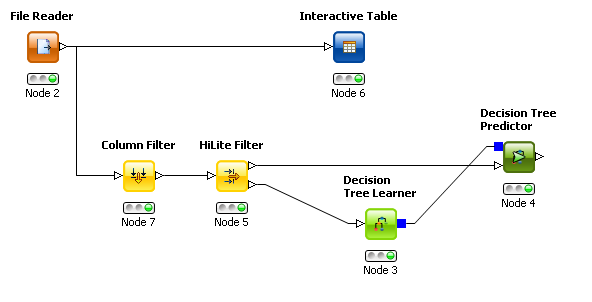
\includegraphics[scale=0.5]{Image/workflowprediction}
		\caption{Workflow de prédiction pour les cas Bulgare et Roumain}
	\end{center}
\end{figure}

 
%----------------------------------------------------

\end{document}
